\documentclass[twoside,11pt]{article}
\usepackage{graphicx,amsmath,latexsym,amssymb}
\usepackage{tikz}
\usepackage{mathdots}
\usepackage[plainpages=false,pdfpagelabels,colorlinks=false,urlcolor=black,pdfpagemode=UseNone,pdfstartview=FitH]{hyperref}
\usepackage{amsthm}
\usepackage{cleveref}
\usepackage{verbatim} %commenting package
\usepackage{subcaption}
\usepackage{float}
\textwidth 12.5truecm \textheight 19truecm \headsep0.5cm
\oddsidemargin 0.6cm \evensidemargin 1cm \topmargin 1cm


% Heading-------------------------------------------------------------------
\markboth{Your Name }
         {\small{Graph Theory Definitions}}
\date{}

% THEOREM Environments ---------------------------------------------------
\newtheorem{theorem}{Theorem}[section]
\newtheorem{lemma}[theorem]{Lemma}
\newtheorem{proposition}[theorem]{Proposition}
\newtheorem{definition}[theorem]{Definition}
\newtheorem{corollary}[theorem]{Corollary}
\newtheorem{example}[theorem]{Example}
\newtheorem{remark}[theorem]{Remark}
\renewcommand{\theequation}{\thesection.\arabic{equation}}
\renewcommand{\thelemma}{\thesection.\arabic{lemma}}
\renewcommand{\theproposition}{\thesection.\arabic{proposition}}
\renewcommand{\thecorollary}{\thesection.\arabic{corollary}}

\makeatletter
\renewcommand*\env@matrix[1][*\c@MaxMatrixCols c]{%
  \hskip -\arraycolsep
  \let\@ifnextchar\new@ifnextchar
  \array{#1}}
\makeatother


% MATH -------------------------------------------------------------------
\newcommand{\p}{\partial}
\newcommand{\bR}{{\bf R}}
\newcommand{\bC}{{\bf C}}
\newcommand{\bZ}{{\bf Z}}
\newcommand{\bN}{{\bf N}}
\newcommand{\bQ}{{\bf Q}}
\newcommand{\bK}{{\bf K}}
\newcommand{\bI}{{\bf I}}
\newcommand{\bv}{{\bf v}}
\newcommand{\bV}{{\bf V}}
\newcommand{\cF}{{\mathcal F}}
\newcommand{\cA}{{\mathcal A}}
\newcommand{\cB}{{\mathcal B}}
\newcommand{\cC}{{\mathcal C}}
\newcommand{\cL}{{\mathcal L}}
\newcommand{\cX}{{\mathcal X}}
\newcommand{\cY}{{\mathcal Y}}
\newcommand{\cZ}{{\mathcal Z}}
\newcommand{\abs}[1]{\left\vert#1\right\vert}
 \newcommand{\set}[1]{\left\{#1\right\}}
 \newcommand{\seq}[1]{\left<#1\right>}
 \newcommand{\norm}[1]{\left\Vert#1\right\Vert}
 \newcommand{\essnorm}[1]{\norm{#1}_{\ess}}
\newtheorem{thm}{Theorem}[section]
\newtheorem{lem}[thm]{Lemma}
\newtheorem{cor}[thm]{Corollary}
\newtheorem{prop}[thm]{Proposition}
\newtheorem{rem}[thm]{Remark}
\newtheorem{ex}[thm]{Example}
\newtheorem{de}[thm]{Definition}

\def\lf{\left\lfloor}
\def\rf{\right\rfloor}

\newenvironment{pf}
    {{\noindent  \textrm{\textbf{Proof }}}~~}

\numberwithin{equation}{section} \DeclareMathOperator{\Var}{Var}
\DeclareMathOperator{\Ima}{Im}
\DeclareMathOperator{\sgn}{sgn}

\newcommand{\N}{{\mathbb{N}}}
\newcommand{\UU}{\widetilde{U}(F)}
\newcommand{\bpf}{\begin{proof}}
\newcommand{\epf}{\end{proof}}
\newcommand{\bpr}{\begin{proposition}}
\newcommand{\epr}{\end{proposition}}
\newcommand{\bdf}{\begin{definition}}
\newcommand{\edf}{\end{definition}}
\newcommand{\blm}{\begin{lemma}}
\newcommand{\elm}{\end{lemma}}
\newcommand{\bex}{\begin{example}\rm }
\newcommand{\eex}{\end{example}}
\newcommand{\bcor}{\begin{corollary}}
\newcommand{\ecor}{\end{corollary}}
\newcommand{\bthm}{\begin{theorem}}
\newcommand{\ethm}{\end{theorem}}

\newcommand{\be}{\begin{enumerate}}
\newcommand{\ee}{\end{enumerate}}
\newcommand{\bq}{\begin{equation}}
\newcommand{\eq}{\end{equation}}
\newcommand{\bb}{\begin{itemize}}
\newcommand{\eb}{\end{itemize}}
\newcommand{\bpw}{\begin{cases}}
\newcommand{\epw}{\end{cases}}
\newcommand{\B}[1]{\textbf{#1}}
\newcommand{\tn}[1]{\textnormal{#1}}
\newcommand{\bs}{\backslash}
\newcommand{\e}{{\epsilon}}
\newcommand{\gs}{{\sigma}}
\newcommand{\ve}{{\varepsilon}}
\newcommand{\bfrac}[2]{\displaystyle \frac{#1}{#2}}
\newcommand{\ds}[1]{\displaystyle {#1}}
\newcommand{\dsum}[2]{\ds{\sum_{#1}^{#2}} }
\newcommand{\ora}[1]{\overrightarrow{#1}}
\newcommand{\ra}{\rightarrow}
\newcommand{\Z}{{\mathbb Z}}

\newtheorem{result}{Result}
% -------------------------------------------------------------------
\begin{document}
\hypersetup{pageanchor=false}
\thispagestyle{empty}
% ---------------------TITLE----------------------------------

\centerline {\bf Counting Trees and Forests in Graphs using Handles}

\vskip.2cm

\centerline{ Lanjing Bao, Patrick Graham}
\centerline{\today}

\begin{abstract}


This paper uses the Matrix-Tree Theorem to explore the effect that modifying simple graphs by adding handles has on the number of directed spanning trees rooted at a vertex. We define two different types of handles for the first time in this paper:
the first one is called a directed handle which consists of a directed edge; the second one is called a directed vertex handle which consists of two directed edges and a vertex.
 Using the Matrix Tree Theorem, we express the number of directed spanning trees by a linear combination of trees and forests of other modified graphs. In particular, we modified an arbitrary simple graph by adding n handles where \(n = 1,2,3\) to discover the number of 2-forests of a graph where 2 vertices are in one tree and one is in the other. We also discover the number of 3-forests where 2 vertices are in one tree and the other two contained in two separate trees.
We further conjecture a similar relationship to count the number of spanning trees in 3-handle graphs.
\end{abstract}


\section{Introduction to Graphs and Handles}

A graph is a finite number of points connected by edges, and a simple graph is a graph with no loops and no parallel edges. A graph can also be categorized as directed or undirected graph. We can also extract part of a graph, such as a spanning tree. Furthermore, we can find out the exact number of spanning trees in a graph using the Matrix Tree Theorem.

\begin{comment}
   This paper is address to undergraduate mathematics majors with little to no knowledge of graph theory. A graph is a finite number of points connected by edges. Given a graph \(G\) you can represent \(G\) as a matrix, such as the Laplacian matrix. We know, from the Matrix-Tree Theorem, that the minor of the Laplacian matrix of \(G\) gives the number of spanning trees. 
\end{comment}
 
   Our paper explores the effect that modifying graphs by adding handles (as shown in Figure 1) has on the number of spanning trees and $n-$forests. We also explore how we can express the number of trees by a linear combination of trees and forests of other modified graphs. Specifically, we modified an arbitrary simple graph by adding $n$ handles, where $n=1,2,3$, and we investigate scenarios of counting the number of spanning trees and $n-$forest in such modified graphs with different roots. 
   
   \begin{figure}[H]
\begin{subfigure}{.5\textwidth}
  \centering
  % include first image
  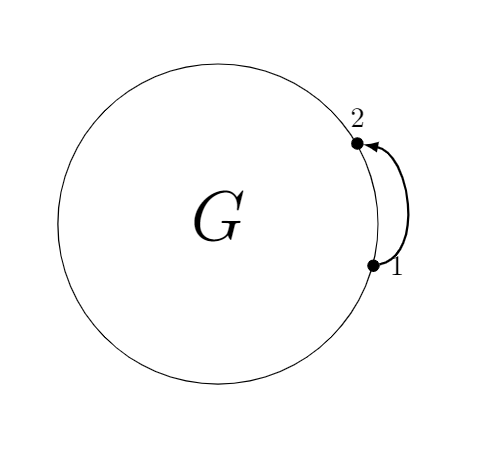
\includegraphics[width=.4\linewidth]{tik_handle_graph.PNG}  \caption{Handle Graph}
\end{subfigure}
\begin{subfigure}{.5\textwidth}
  \centering
  % include second image
  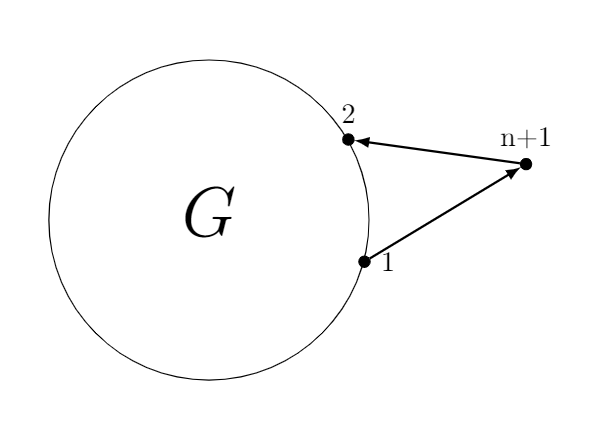
\includegraphics[width=.5\linewidth]{tik_vertex_handle_graph.PNG}  \caption{Vertex Handle Graph}
\end{subfigure}
\caption{Modified Graphs by Adding 1 Handle.}
\label{fig:H_VH}
\end{figure}
   
   Finally, we discover that the number of 2-forests of a graph where 2 vertices are in one tree and one is in the other for any 3 vertices of a graph is a linear combination of the numbers of spanning trees rooted at different vertices. Similarly, we can find the number of three forests of a graph where 2 vertices are in one tree and the other two vertices are in two different trees.

\section{Graphs and Trees}
We first introduce definitions and properties about graphs, such as digraph, subgraph, and spanning tree, in the first part of this section. In the second part of the section, we further examine how to convert a graph into a matrix.

\subsection{Definitions of Graph}

\bdf
{\bf (Graph)}\\
A {\it graph}, $G$, consists of a vertex set $V(G)=\{v_1, v_2, \dots, v_n\}$ and an edge set $E(G)\subseteq \{\{x, y\}\textrm{ or } (x,y) |\ x, y \in V(G) \text{where}\ x \neq y \}$. 
\edf

This means, the edge set may consist of directed edges or undirected edges: the ordered pair $(x,y)$ denotes a directed edge from $x$ to $y$, and the unordered pair $\{x,y\}$ denotes a undirected edge between $x$ and $y$.
Additionally, the order of $G$ is the number of vertices in $G$, $|V(G)|$.

In our paper, we will be using natural numbers instead of labeled vertices. For example, we will write vertex $v_1$ as 1 and a set of vertices $\{v_1,v_2,...,v_n\}$ as $\{1,2,...,n\}$. 

Next, we are going to introduce a special category of graphs, digraph.

\bdf
{\bf (Digraph)}
A {\it directed graph} or {\it digraph} is a graph where all edges are directed.
\edf
Similarly, a graph is called a undirected graph if all the edges in the graph are undirected.

Moreover, a {\it directed path,} $\ora{P}_m,$ $m\geq 1$ is a digraph with $m$ vertices, a vertex set
 $V(\ora{P}_m)=\{1,2,...,m\}$, and an edge set
 $E(\ora{P}_m)=\{(1,2),(2,3),...,(m-1,m)\}.$ For instance, the following digraph is a directed path:
$$\overset{1}{\bullet}\ra \overset{2}{\bullet} \ra \cdots \ra \overset{m}{\bullet}$$

On the other hand, a {\it path graph } ${P_m},$ $m\geq 1$ is a undirected graph with $m$ vertices, vertex set $V({P_m})=\{1,2,...,m\}$ and an edge set $E({P_m})=\{\{1,2\},\{2,3\},...,\{m-1,m\}\}$. For instance, the following undirected graph is a path graph:
$$\overset{1}{\bullet}\leftrightarrow \overset{2}{\bullet} \leftrightarrow \cdots \leftrightarrow \overset{m}{\bullet}$$

Another type of graph is cycle graph. A {\it cycle graph } ${C_m},$ $m\geq 3$ is a undirected graph with $m$ vertices, vertex set  $V({C_m})=\{1,2,...,m\}$ and an edge set $E({C_m})=\{\{1,2\},\{2,3\},...,\{m-1,m\}, \{m,1\}\}$. Similarly, a {\it directed cycle } $\ora{C}_m,$ $m\geq 2$ is a digraph with $m$ vertices, a vertex set
$V(\ora{C}_m)=\{1,2,...,m\}$ and an edge set $E(\ora{C}_m)=\{(1,2),(2,3),...,(m-1,m),(m,1)\}.$ Here is a comparison of cycle graph and directed cycle.

\begin{figure}[H]
\begin{subfigure}{.5\textwidth}
  \centering
  % include first image
  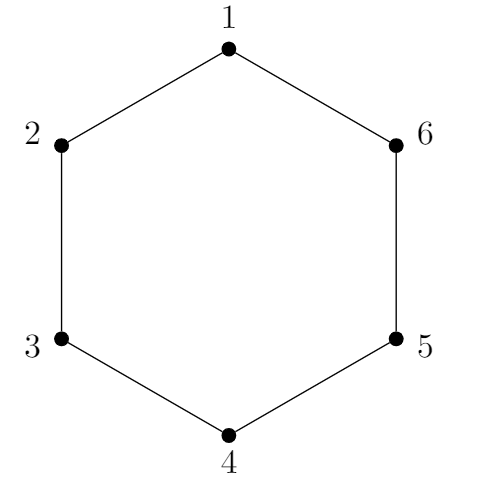
\includegraphics[width=.8\linewidth]{tik_undirected_c6.PNG}  
  \caption{Cycle graph $C_6$}
  \label{fig:sub-first}
\end{subfigure}
\begin{subfigure}{.5\textwidth}
  \centering
  % include second image
  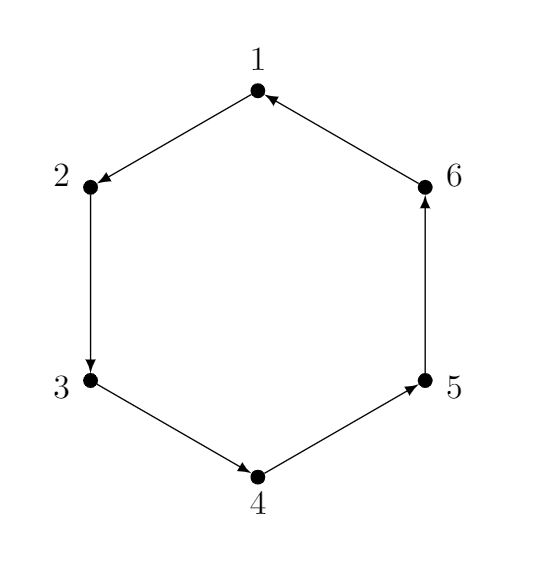
\includegraphics[width=.8\linewidth]{tik_c6.PNG}  
  \caption{Directed cycle $\ora{C}_m$}
  \label{fig:sub-second}
\end{subfigure}
%\label{fig:fig}
\end{figure}

Given an arbitrary graph, we can modify the graph by adding an edge or a directed path. In our paper, the following two special types of  modified graphs, directed handle graph and directed vertex handle graph (as shown in Figure 1), are the main objects we study and explore.

\bdf {\bf{(Directed Handle Graph)}}
For a graph $G$ of order $m$ and vertices $u,v\in V(G)$, we denote $G_{(u,v)}$ to be the graph where a directed edge from vertex $u$ to vertex $v$ is added to $E(G)$.
\edf

 We refer to this as the directed graph handle $(u,v)$. Furthermore, we refer to the starting node $u$ as the outflow point, and $v$ is referred to as the inflow point with $u$ and $v$ being handle pairs. In the case that multiple handles are added $G_{(u_{1},v_{1}),(u_{...},v_{...}),(u_{n},u_{n})}$ will represent the handles of the graph being added. This will also be referred to as $H_{n}(G)$. We also will relabel $H_{n}(G)$ as 
 $(G)_{(1,2),(...,...),(n-1,n)}$ for ease as well as we know that the number of spanning trees invariant.

\bdf {\bf{(Directed Vertex Handle Graph)}}
Let $G=(V,E)$ be a graph, and $u,v\in V(G)$. We denote $VH(G)$ as a graph where a new vertex $w\notin V(G)$ and two directed edges, $e_1=(u,w)$ and $e_2=(w,v)$ are added to $V(G)$. In symbols, $VH(G):= (V(G)\cup \{w\},\; E(G)\cup \{e_1,e_2\})$.
\edf

To extract part of a graph, we are going to define subgraph, directed rooted tree, and spanning tree.
\bdf
{\bf (Subgraph)}
Let $G= (V,E)$ be a digraph.  We say $H= (U,F)$ is a subgraph of $G$ if $F \subseteq E$ or \(U \subseteq V\).  In case of $V(G)=V(H)$, we call $H$ a spanning subgraph of $G$.
\edf

\bdf
{\bf (Directed  Rooted Tree)}
Let $G=(V,E)$ be a graph with $|V|=n$ and $v_i \in V(G)$, where $i$ is an integer with $1\leq i \leq n$.
We say a subgraph $T$ of $G$ is a directed  rooted tree or tree rooted at $i$, if there is a unique path from $i$ to $j$ for all $j=1,...,i-1,i+1,...n$.
\edf

\bdf
{\bf (Spanning Tree)}
Let $G=(V,E)$ be a graph. A tree $T$ in $G$ is a spanning tree if $V(T)= V(G)$. 
\edf

% Make a paragraph stating what a directed spanning tree rooted is and its purpose

Notice, a directed tree is not necessarily a directed spanning tree. When the directed rooted tree $T$ consists of all the vertices in $G$, $T$ is a  directed spanning tree. In our paper,
We will be counting the number of directed spanning trees rooted at a vertex v in the directed handle graph and directed vertex handle graph with $n$ handles, where $n=1,2,3$.

\subsection{Converting Graphs into Matrices}
Now that we have discussed what digraphs are and several examples of digraphs as well as directed spanning trees rooted at a vertex, we are going to turn graphs into matrices to uncover more information about the graph.
\bdf
{\bf (Adjacency Matrix)}
Let $G$ be a graph. The {\it adjacency matrix} of the graph is the
$n \times n$ matrix $A(G) = [a_{ij}]_{n \times n}$
such that
\begin{displaymath}
a_{ij} =  \left\{\begin{array}{ll} 1 & \textrm{if $ \{v_i, v_j\} \textrm{ or } (v_i,v_j) \in E(G)$ }
 \\ 0 & \textrm{otherwise }
\end{array}\right.
\end{displaymath}
We denote {\it the determinant of a graph} $G$ as $det(A(G))=|G|$.
\edf

\bdf
{\bf (Degree of Vertex)}
Let $G=(V,E)$ be a graph, and let $v\in V(G)$.
The {\it degree} of \(v\) is the number of edges attached to \(v\), denoted as \(deg(v)\).
\edf
In our paper, the graph we mainly consider is formed by adding directed handles onto a undirected graph. To count the number of spanning trees in such graph, we need to further distinguish types of edges attached to the vertex. Therefore, we define
the {\bf indegree} of a vertex \(v\) as the number of  directed edges going into \(v\), denoted as \(deg^{-}(v)\), and 
the {\bf outdegree} of \(v\) as the number of directed edges going out of \(v\), denoted as \(deg^{+}(v)\). 

It follows that \(deg(v)=deg^{-}(v)+deg^{+}(v)\).

\bdf
{\bf (Degree Matrix)}
Let $G=(V,E)$ be a graph with $|V(G)|=n$. The {\it degree matrix} is a $n\times n$ diagonal matrix $D(G) = [d_{ij}]_{n \times n}$ such that
\begin{displaymath}
d_{ij} :=  \left\{\begin{array}{ll} deg(v_i) & \textrm{if $i=j$ }
 \\ 0 & \textrm{otherwise }
\end{array}\right.
\end{displaymath}
\edf
For the same reason we differentiate indegree and outdegree vertex, we further distinguish indegree matrix and outdegree matrix base on the direction of the edge attached to the vertex. 

Formally, 
let $G=(V,E)$ be a digraph with $|V(G)|=n$. The {\bf indegree matrix} is a $n\times n$ diagonal matrix $ID(G) = [d_{ij}]_{n \times n}$ such that
\begin{displaymath}
d_{ij} :=  \left\{\begin{array}{ll} deg^{-}(v_i) & \textrm{if $i=j$ }
 \\ 0 & \textrm{otherwise }
\end{array}\right.
\end{displaymath}

Analogously, we denote the {\bf outdegree matrix} as a $n\times n$ diagonal matrix such that \(d_{ij} = deg^{+}(v_i)\) if $i=j$, and $0$ otherwise.

\bdf
{\bf (Laplacian Matrix)}
Let $G=(V,E)$ be a graph with $|V(G)|=n$. The {\it Laplacian matrix} is a $n\times n$ diagonal matrix $L(G)$ defined as
$$ L(G)=D(G)-A(G)  $$
\edf

We define directed spanning trees rooted at a vertex to have directed paths from the root, then we need the \(deg^{-}(v)\).

An {\bf In-Laplacian Matrix} is a $n\times n$ diagonal matrix IL$(G)$ defined as
$$ IL(G)=ID(G)-A(G)  $$

Lastly, we are going to introduce a special matrix operation to get the minor of a matrix.
\bdf
{\bf (Minor)}
Let $G=(V,E)$ be a graph with $|V|=n$. The {\it minor} of $G$ is a $(n-1)\times (n-1)$ diagonal matrix obtained by removing the $i$th row and column from $G$, denoted as $Minor(G)$.
\edf

\section{Matrix Tree Theorem for Digraph}
With the preparation in section 1, we are ready to understand the Matrix Tree Theorem. 

\bthm\cite{leenheer}
{\bf Matrix-Tree Theorem for Digraphs} 
Let $G = (V,E)$ be a digraph. Then the number of
directed spanning rooted trees at $v$ equals to the determinant of the minor of the In-Laplacian of $G$, \(Minor(L(G)_i)\) where $i$ is the \(ii\) entry where the root $v$ is.
\ethm

Here is an example of using the Matrix-Tree Theorem for Digraphs. 

\bex
Let $G$ be a cycle graph, $C_6$. Let $G'=\{V(C_6)\cup \{7\}, E(C_6)\cup \{(6,7),(7,2)\}$.

\begin{figure}[H]
  \centering
  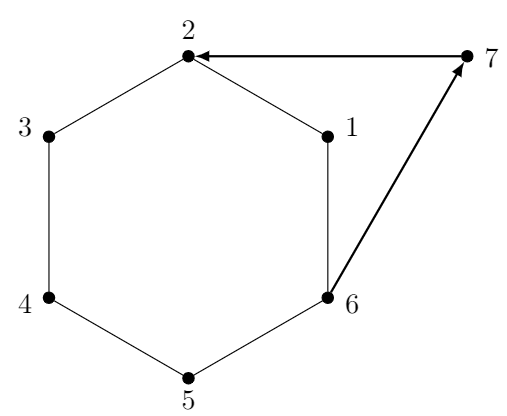
\includegraphics[scale=0.5]{tik_example.PNG}  
\end{figure}

Then the indegree matrix and adjacency matrix of $G'$ are \[ ID(G')=
\begin{bmatrix}
2 & 0 & 0 & 0 & 0 & 0 & 0\\
0 & 3 & 0 & 0 & 0 & 0 & 0\\
0 & 0 & 2 & 0 & 0 & 0 & 0\\
0 & 0 & 0 & 2 & 0 & 0 & 0\\
0 & 0 & 0 & 0 & 2 & 0 & 0\\
0 & 0 & 0 & 0 & 0 & 2 & 0\\
0 & 0 & 0 & 0 & 0 & 0 & 1
\end{bmatrix},\; A(G')=
\begin{bmatrix}
0 & 1 & 0 & 0 & 0 & 1 & 0\\
1 & 0 & 1 & 0 & 0 & 0 & 1\\
0 & 1 & 0 & 1 & 0 & 0 & 0\\
0 & 0 & 1 & 0 & 1 & 0 & 0\\
0 & 0 & 0 & 1 & 0 & 1 & 0\\
1 & 0 & 0 & 0 & 1 & 0 & 1\\
0 & 1 & 0 & 0 & 0 & 1 & 0
\end{bmatrix}
\]
Then the in-Laplacian matrix of $G'$ is $IL(G')=ID(G')-A(G')$, 

\begin{equation*} 
\begin{split}
IL(G') & = 
\begin{bmatrix}
2 & 0 & 0 & 0 & 0 & 0 & 0\\
0 & 3 & 0 & 0 & 0 & 0 & 0\\
0 & 0 & 2 & 0 & 0 & 0 & 0\\
0 & 0 & 0 & 2 & 0 & 0 & 0\\
0 & 0 & 0 & 0 & 2 & 0 & 0\\
0 & 0 & 0 & 0 & 0 & 2 & 0\\
0 & 0 & 0 & 0 & 0 & 0 & 1
\end{bmatrix} - 
\begin{bmatrix}
0 & 1 & 0 & 0 & 0 & 1 & 0\\
1 & 0 & 1 & 0 & 0 & 0 & 1\\
0 & 1 & 0 & 1 & 0 & 0 & 0\\
0 & 0 & 1 & 0 & 1 & 0 & 0\\
0 & 0 & 0 & 1 & 0 & 1 & 0\\
1 & 0 & 0 & 0 & 1 & 0 & 1\\
0 & 1 & 0 & 0 & 0 & 1 & 0
\end{bmatrix} \\
 & = \begin{bmatrix}
2 & -1 & 0 & 0 & 0 & -1 & 0\\
-1 & 3 & -1 & 0 & 0 & 0 & -1\\
0 & -1 & 2 & -1 & 0 & 0 & 0\\
0 & 0 & -1 & 2 & -1 & 0 & 0\\
0 & 0 & 0 & -1 & 2 & -1 & 0\\
-1 & 0 & 0 & 0 & -1 & 2 & -1\\
0 & -1 & 0 & 0 & 0 & -1 & 1
\end{bmatrix}
\end{split}
\end{equation*}

By removing the $6^{th}$ row and $6^{th}$ column, the minor of the in-Laplacian of $G'$ at 6  is
\[Minor(IL(G')_6)=
\begin{bmatrix}
2 & -1 & 0 & 0 & 0  & 0\\
-1 & 3 & -1 & 0 & 0 &  -1\\
0 & -1 & 2 & -1 & 0 &  0\\
0 & 0 & -1 & 2 & -1 &  0\\
0 & 0 & 0 & -1 & 2 &  0\\
0 & -1 & 0 & 0 & 0 &  1
\end{bmatrix}
\]
Using Mathematica to calculate the determinant of $Minor(IL(G')_6)$, we have $|Minor(IL(G')_6)|=6$.
Therefore, by the Matrix Tree Theorem for Digraph, there are 6 directed spanning trees rooted at $6$. 

We note that relabeling the vertices does not change the number of spanning trees that are rooted at the same vertex. For example, we can relabel $G'$ as following: 
\begin{figure}[H]
     \centering
     \begin{subfigure}[b]{0.4\textwidth}
         \centering
         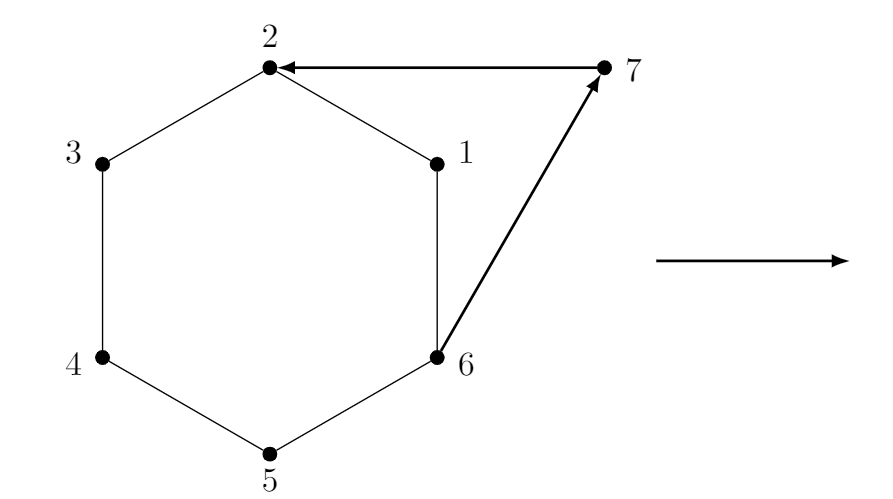
\includegraphics[width=\textwidth]{tik_example1.PNG}
     \end{subfigure}
     \begin{subfigure}[b]{0.3\textwidth}
         \centering
         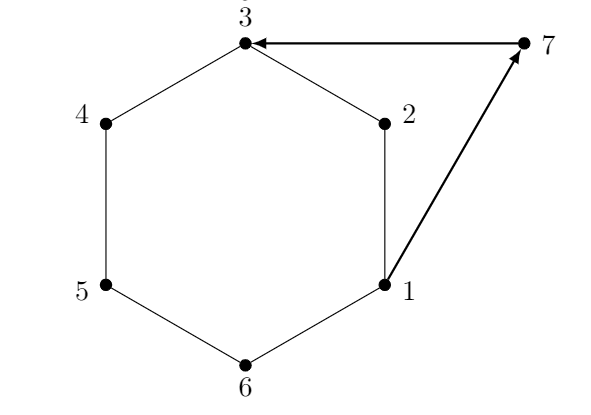
\includegraphics[width=\textwidth]{tik_example2.PNG}
     \end{subfigure}
\end{figure} 
Using the Matrix Tree Theorem for Digraph to calculate the number of directed spanning trees rooted at $1$, $|Minor(IL(G')_1)|=6$.
\eex

\section{Explorations}
Inspired by the work of Gyurov and Pinzon\cite{GP} where they used handle graphs to find determinants of joined graphs, we consider two types of modified graphs in this paper: directed handle graphs and directed vertex handle graphs (as shown in Figure. \ref{fig: H_VH}). Using the Matrix Tree Theorem for Digraphs, we are able to find the linear combination of the number of spanning trees in the subgraph and the number of $n-$forest. 

\begin{figure}[H]
\begin{subfigure}{.5\textwidth}
  \centering
  % include first image
  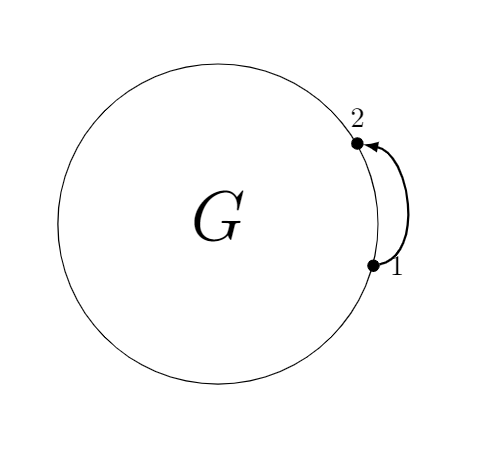
\includegraphics[width=.4\linewidth]{tik_handle_graph.PNG}  \caption{Handle Graph}
\end{subfigure}
\begin{subfigure}{.5\textwidth}
  \centering
  % include second image
  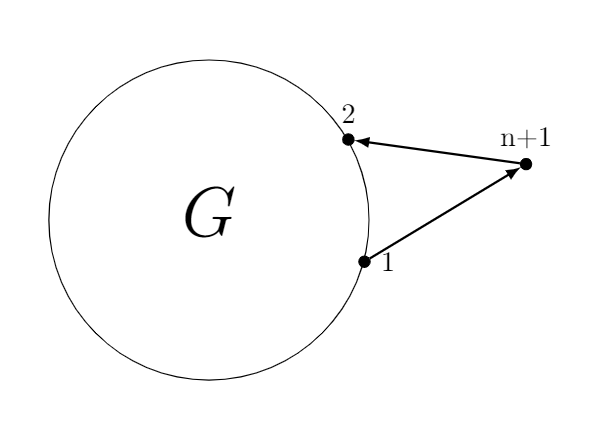
\includegraphics[width=.5\linewidth]{tik_vertex_handle_graph.PNG}  \caption{Vertex Handle Graph}
\end{subfigure}
\caption{Comparison of Handle Graph and Vertex Handle Graph}
\label{fig: H_VH}
\end{figure}

In this section, we first examine the relation between the number of spanning trees and the $n-$spanning forests, and we discover that the number of the spanning trees does not change when adding an edge to a vertex in a graph by creating a bijection. Then, we continue to explore the linear relationship between the number of the spanning trees and the number of $n-$forests rooted at different nodes in the handle graph and vertex handle graph with 1 and 2 handles, respectively.

\subsection{Bijection between spanning trees and number of n- spanning forests}

In this section, we are going to explore some bijection relations between the spanning trees and number of $n$-spanning forests in our directed handle graphs and directed vertex handle graph. 

We first introduce some terminology. Let $G$ be a graph. A {\bf path} from vertex x to vertex y in $G$ is a directed path graph that is a subgraph of $G$ that begins at $x$ and ends at $y$. Moreover, $x$ is said to be {\bf connected} to $y$ if there exists a path from $x$ to $y$.

In the following lemma, we are going to show that the outflow vertex cannot be connected by a path to the inflow vertex in $G$ when a spanning tree contains the handle.
\blm
\label{symhandle}
Let $VH_n(G)$ be a directed vertex handle graph of $G$ with $n$ handles. Let $r$ be the outflow vertex of one of the handles, and let $v$ be the inflow vertex of the same handle.
Let $T$ be a spanning tree in $VH_n(G)$ such that $T$ is rooted at $r$. Then there does not exist a path $p\in G$ from $r$ to $v$. 
\elm

\bpf
Let $VH_n(G)$ be a directed vertex handle graph of $G$ with $n$ handles. Let $r$ be the outflow vertex of one of the handles, and let $v$ be the inflow vertex paired with $r$.
Let $T$ be a spanning tree in $VH_n(G)$ such that $T$ is rooted at $r$.  Suppose there exists a path $p\in G$ from $r$ to $v$. By definition of spanning tree, there exists a directed path $p'$ from the root $r$ using the inflow edge and outflow edge to $v$. But this contradicts with our assumption that $T$ is a spanning tree because the path $p$ and $p'$ will create a cycle in $T$. Therefore, there does not exists a path in $G$ from the outflow vertex to the inflow vertex.
\epf

Let $G$ be a group. From now on, we denote $\tau(G)$ as the number of trees in $G$ and $T (G)$ as the set of all spanning tree in $G$. 

In the next lemma, we want to show that adding one outflow edge to a outflow vertex does not change the number of spanning trees in the graph. In order to show this, recall any two finite sets $A,B$, $|A|=|B|$ if and only if there is a bijection from $A$ to $B$. Therefore, we only need to show there exists a bijection between $T(G)$ and $T(G')$.

\blm
\label{bij_count}
Let $G=(V,E)$ be a graph, and let $v'$ be a vertex such that $v'\notin V(G)$. Let a graph $G':= (V(G)\cup \{v'\}, E(G)\cup \{e\})$, with  $e$ being a directed edge from some vertex $v\in V(G)$ to $v'$. Then $\tau(G)=\tau(G')$.
\elm
\begin{figure}[H]
    \centering
    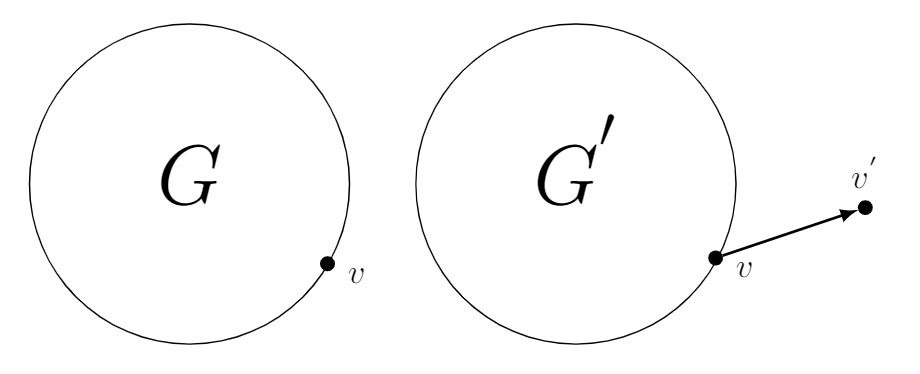
\includegraphics[scale=0.5]{tik_bijec.PNG}
\end{figure}
\bpf
Let $G=(V,E)$ be a graph, and let $v'$ be a vertex such that $v'\notin V(G)$. Let a graph $G':= (V(G)\cup \{v'\}, E(G)\cup \{e\})$, with  $e$ being a directed edge from some vertex $v\in V(G)$ to $v'$. 

Define function $f: T(G)\rightarrow T(G')$. The function $f$ maps any spanning tree $t\in T(G)$ to a tree $t'\in T(G')$ by adding the directed edge $e$ to the vertex $v$. 

We know $t'$ is also a spanning tree because by adding an external edge does not create a cycle and $t'$ is also a spanning tree. 

To show $f^{-1}$ is defined, let $t'$ be a spanning tree in $G'$. By deleting the edge $e$ and the vertex $v'$ from the spanning tree $t'$, we get another spanning $t$ and $t$ is in $G$ because all of the vertices are used in $G$ and there is not a cycle in $t$. Therefore, $f^{-1}$ is defined. 

To show each pre-image of $t'$ is also unique, for each $t'\in T(G')$, there is only one tree $t$ by deleting the edge $e$. We know $t$ is a spanning tree in $T(G)$ because $V(t)=V(G)$. Therefore, for each spanning tree $t'\in G'$, there is a unique pre-image $t\in G$. 

Thus, the function $f$ is a bijection. Therefore, the cardinality of $T(G)$ equals to the cardinality of $T(G')$, that is $|T(G)|=|T(G')|$.

Therefore, the number of spanning in $G$ equals the number of spanning in $G'$, that is $\tau(G)=\tau(G')$.
\epf

\bdf
{\bf ($n$-Forest)}
Let $G=(V,E)$ be a graph. If $G$ is partitioned into $n$ directed trees, $G_1, G_2, ..., G_n$ such that $V(G_1)\cap V(G_2) \cap ... \cap V(G_n)=\emptyset$ and each $G_i$ for $i$ from 1 to $n$ is a directed rooted tree, then we say the graph is a $n$-forest, denoted $T_{(1)(2)...(n)}(G)$.
\edf
*vgv\blm
\label{bij_handle}
Let $G=(V,E)$ be a graph, and let $v'$ be a vertex such that $v'\notin V(G)$. Let $v_1,v_2$ be two distinct vertices in $G$. Suppose a graph $G'=(V(G)\cup \{v\},E(G)\cup \{e_1,e_2\})$ where $e_1$ is an outflow edge from $v_1$ to $v$, and $e_2$ is an inflow edge from $v$ to $v_2$. Then $\tau(G')=\tau(G)+\tau_{(1)(2)}(G)$.
\elm
\begin{figure}[H]
    \centering
    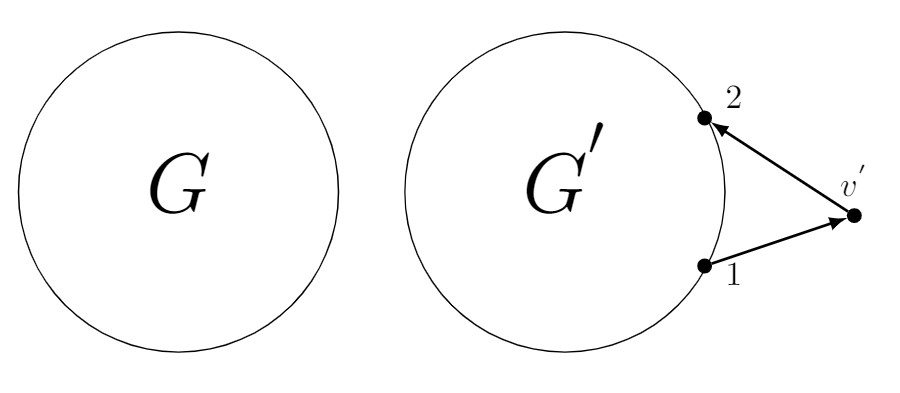
\includegraphics[scale=0.4]{tik_handle_bijec.PNG}
\end{figure}
\bpf
Let $G=(V,E)$ be a graph, and let $v'$ be a vertex such that $v'\notin V(G)$. Let $v_1,v_2$ be two distinct vertices in $G$. Suppose a graph $G'=(V(G)\cup \{v'\},E(G)\cup \{e_1,e_2\})$ where $e_1$ is an outflow edge from $v_1$ to $v$, and $e_2$ is an inflow edge from $v$ to $v_2$.

Let $t'$ be a spanning tree in $T(G')$. There are two types of spanning trees rooted at $v_1$: $e_2\in E(t')$ or $e_2\notin E(t')$. 

Case 1: $e_2\notin E(t')$. 

By the \Cref{bij_count}, $\tau(G)=\tau(G')$. 

Case 2: $e_2\in E(t')$. 

To show the number of the spanning trees rooted at $v_1$ in $G'$ equals to the number of spanning trees in the two-forest rooted at $v_1$ and $v_2$, define a function $f: T(G')\rightarrow T_{(1)(2)}(G)$. 

Let $t$ be a two-forest rooted at $v_1,v_2\in V(G)$. So, there not exists a path between $v_1$ and $v_2$. By adding a vertex $v\notin G$, a directed edge $e_1$ from $v_1$ to $v$, and another directed edge $e_2$ from $v$ to $v_2$, we form a spanning tree $g'$. Since $t'$ is a spanning tree, $t'\in G'$. Therefore, $f^{-1}$ is defined. So, $f$ is a bijection. Thus, $\tau(G')=\tau_{(1)(2)}(G)$.

Thus, combining two cases, $\tau(G')=\tau(G)+\tau_{(1)(2)}(G)$.

\epf

Our exploration of graph theory was first looking at the operation of adding an arbitrary directed handle to any two points of a graph. We have gain some insights by observing its effects below.  

\subsection{Graphs with 1 handle}

We first started looking at how to classify the number of directed spanning trees of any graph rooted at a specific vertex by adding a single directed handle to the graph. First, we can relabel the graph such that the outflow vertex is 1 and the inflow vertex is 2. This is important because our proofs will follow this labeling for ease and consistency. 

\subsubsection{Graphs with 1 handle rooted at 1}
We will specify the rooting of this graph at vertex one which is the outflow vertex. now let us see how to classify the trees of this graph. And from now on we mean spanning directed trees rooted at a vertex v.

\bthm
Let $G$ be undirected simple graph, and let $VH_1(G)$ be directed handle graph of $G$ with 1 handle. 
\begin{figure}[H]
    \centering
    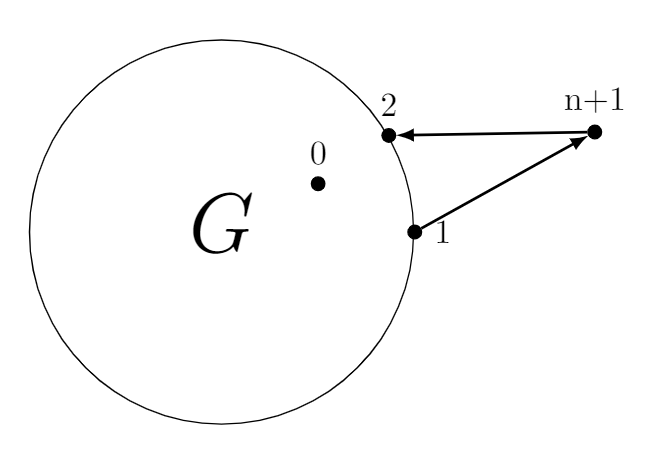
\includegraphics[scale=0.3]{tik_1handle.PNG}
\end{figure}
Then the number of spanning trees that are rooted at 1 in $VH_1(G)$ equals to the number of spanning trees in $G$ plus the number of 2-forests rooted at 1 and 2 in $G$ \[
 \tau_1(VH_1(G)) = \tau(G)+\tau_{(1)(2)}(G)
\]
\ethm

\bpf
Let $G$ be undirected simple graph, and
let $VH_1(G)$ be directed handle graph of $G$ with 1 handle. Let $t$ be a spanning tree in $VH_1(G)$. Suppose $t$ is rooted at 1. Let $e$ be the inflow edge. Then, there are two cases.\\
Case 1. $e\notin VH_1(G)$. Then the number of spanning tree is $\tau(G)$ by \Cref{bij_count}.\\
Case 2. $e \in VH_1(G)$. Then, since there does not exist a path in $G$ between node 1 and 2 by \Cref{symhandle}, the number of spanning trees is $\tau_{(1)(2)}(G)$.\\
Therefore, the total number of spanning tress in $VH_1(G)$ is  $$ \tau_1(VH_1(G)) = \tau(G)+\tau_{(1)(2)}(G)$$ .
\epf


\blm\label{DH Rooted at 1}
Let $G$ be undirected simple graph, and let $H_1(G)$ be directed handle graph of $G$ with 1 handle. Then the number of spanning trees that are rooted at 1 in $H_1(G)$ equals to the number of spanning trees in $G$ plus the number of 2-forests rooted at 1 and 2 in $G$ \[
 \bf{\tau_1(H_1(G)) = \tau(G)+\tau_{(1)(2)}(G)} 
\]
\elm

\bpf
Let $G$ be undirected simple graph, and
let $H_1(G)$ be directed handle graph of $G$ with 1 handle. Let $t$ be a tree in $H_1(G)$. Suppose $t$ is rooted at 1. Let $e$ be the handle. Then, there are two cases.\\
Case 1. $e\notin H_1(G)$. Then the number of spanning tree is $\tau(G)$ by \Cref{bij_count}.\\
Case 2. $e \in H_1(G)$. Then, since there does not exist a path in $G$ between node 1 and 2 by \Cref{symhandle}, the number of spanning trees is $\tau_{(1)(2)}(G)$.\\
Therefore, the total number of spanning tress in $H_1(G)$ is  $$ \tau_1(H_1(G)) = \tau(G)+\tau_{(1)(2)}(G)$$ .
\epf

\subsubsection{Graphs with 1 handle rooted at 2}
Now that we have a good introduction into the analysis of the graph we will look at what happens when we root a graph at the vertex two other wise known as the inflow vertex 

\bthm
Let $VH_1(G)$ be directed vertex handle graph with 1 handle.
\begin{figure}[H]
    \centering
    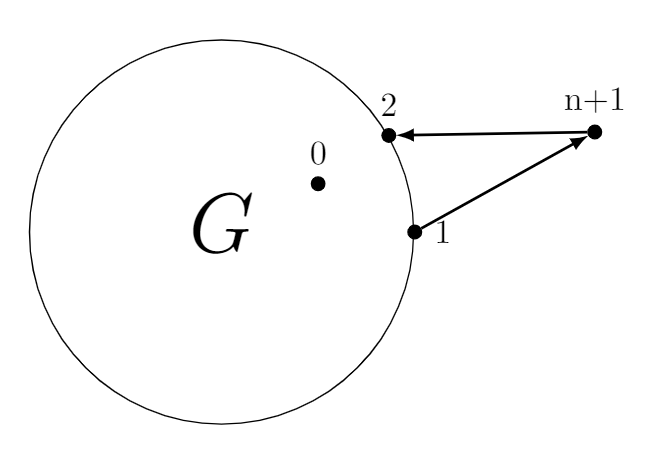
\includegraphics[scale=0.3]{tik_1handle.PNG}
\end{figure}
Then the number of spanning trees that are rooted at 2 in $VH_1(G)$ equals to the number of spanning trees in $G$   \[
 \tau_2 (VH_1(G)) = \tau(G)
\]
\ethm

\bpf
Let $VH_1(G)$ be directed handle graph with 1 handles, and let $t$ be a spanning tree in $VH_1(G)$. Suppose $T$ is rooted at 2. Then the inflow edge $e\notin VH_1(G)$. Then, by \Cref{bij_count}, the total number of spanning tress in $VH_1(G)$ is  $$ \tau_2 (VH_1(G)) = \tau(G)$$.
\epf


\bthm\label{DH rooted 2}
Let $H_1(G)$ be directed handle graph with 1 handle. Then the number of spanning trees that are rooted at 2 in $H_1(G)$ equals to the number of spanning trees in $G$   \[
 \tau_2 (H_1(G)) = \tau(G)
\]
\ethm

\bpf
Let $H_1(G)$ be directed handle graph with 1 handles, and let $t$ be a spanning tree in $H_1(G)$. Suppose $T$ is rooted at 2. Then the inflow edge $e\notin H_1(G)$. Then, by \Cref{bij_count}, the total number of spanning tress in $H_1(G)$ is  $$ \tau_2 (H_1(G)) = \tau(G)$$.
\epf


\subsubsection{Graphs with 1 handle rooted at 0}
Finally we will observe the changes in the trees of this graph when rooting the graph at an arbitrary vertex which is neither the inflow or outflow vertex we will relabel vertex 0. 

\bthm
Let $VH_1(G)$ be directed vertex handle graph with 1 handle. 
\begin{figure}[H]
    \centering
    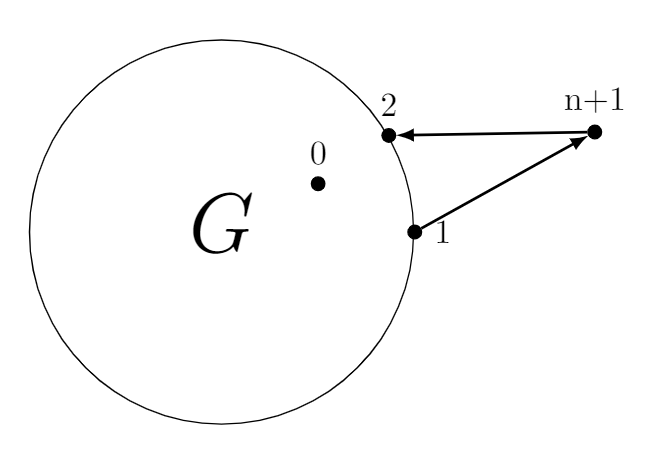
\includegraphics[scale=0.3]{tik_1handle.PNG}
\end{figure}
Then the number of spanning trees that are rooted at 0 in $VH_1(G)$ equals to the number of spanning trees in $G$ plus the number of 2-forest rooted at 0 and 2 in $G$\[
 \tau_0 (VH_1(G)) = \tau(G)+\tau_{(01)(2)}(G) 
\]
\ethm

\bpf
Let $VH_1(G)$ be directed vertex handle graph with 1 handle, and let $t$ be a spanning tree in $VH_1(G)$ and $e$ be the inflow edge.. If $t$ is rooted at 0, there are two cases.

Case 1. $e\notin VH_1(G)$. 

By \Cref{bij_count}, the number of spanning tree is $\tau(G)$ .

Case 2. $e \in VH_1(G)$. 

Then there does not exist a path between node 1 and 2 by \cref{symhandle}. Therefor, the only option is to form a 2-forested rooted at 0 and 2. That is the number of spanning tree is $\tau_{(01)(2)}(G)$.

In conclusion, the total number of subgraphs of $VH_1(G)$ is  \\
$$\tau_0 (VH_1(G)) = \tau(G)+\tau_{(01)(2)}(G)$$ .
\epf

\bthm\label{DH1 rooted at 0}
Let $H_1(G)$ be directed handle graph with 1 handle. Then the number of spanning trees that are rooted at 0 in $H_1(G)$ equals to the number of spanning trees in $G$ plus the number of 2-forest rooted at 0 and 2 in $G$\[
 \tau_0 (H_1(G)) = \tau(G)+\tau_{(01)(2)}(G) 
\]
\ethm

\bpf
Let $H_1(G)$ be directed handle graph with 1 handle, and let $t$ be a tree in $H_1(G)$ and $e$ be the handle. If $t$ is rooted at 0, there are two cases.

Case 1. $e\notin H_1(G)$. 

By \Cref{bij_count}, the number of spanning tree is $\tau(G)$ .

Case 2. $e \in H_1(G)$. 
%I am making a comment to clarify the language better after we submit for semester
Then there does not exist a path between node 1 and 2 by \cref{symhandle}. Therefor, the only option is to form a 2-forested rooted at 0 and 2. That is the number of spanning tree is $\tau_{(01)(2)}(G)$.

In conclusion, the total number of trees of $H_1(G)$ is  \\
$$\tau_0 (H_1(G)) = \tau(G)+\tau_{(01)(2)}(G)$$ .
\epf


% New result
This is a new result! Let $VH_1(G)$ be directed vertex handle graph with 1 handle. Then the number of 2-forest rooted at 0 and 2 equals to the difference between the number of the spanning trees in $VH_1(G)$ and $G$. Moreover, using the Matrix Tree Theorem for digraph, we can calculate the exact number of $\tau_{(01)(2)}(G)$= $\tau_0 VH_1(G) - \tau(G)$.


\bcor
Let $H_1(G)$ be directed handle graph with 1 handle. Then the number of 2-forest rooted at 0 and 2 equals to the difference between the number of the spanning trees in $H_1(G)$ and $G$. Moreover, using the Matrix Tree Theorem for digraph, we can calculate the exact number of $\tau_{(01)(2)}(G)$.
\ecor

\subsection{Graphs with 2 handles}

In this section, we begin with an observation. Let $G$ be a graph with $n$-forest. When a vertex $v\in G$ is not presented in any of the forest, this situation actually covers all cases in which $v$ is in each of the n-forest. For example, the number of 3-forest in $G$ is\\ $\tau_{(1)(2)(4)}(G)=\tau_{(13)(2)(4)}(G)+\tau_{(1)(23)(4)}(G)+\tau_{(1)(2)(43)}(G)$.

\blm
\label{addedW}
Let $G=(V,E)$ be a graph and\\ $V(G)=\{1,2,...,k,k+1,...,p-1,p,...,w\}$.
Then $$\tau_{(1,...,k), (k+1,...,p)}(G)=\tau_{(1,...,k,w)(k+1,...,p)}(G)+\tau_{(1,...,k)(k+1,...,p,w)}(G)$$
with neither $(v_1,...,v_k,w)$ nor $(k+1,...,p,w)$ form cycles.
\elm

\bpf
Let $G=(V,E)$ be a graph and\\ $V(G)=\{1,2,...,k,k+1,...,p-1,p,...,w\}$ and neither $(v_1,...,v_k,w)$ nor $(k+1,...,p,w)$ form cycles in $G$.
Since neither $(v_1,...,v_k,w)$ nor $(k+1,...,p,w)$  form cycles, there are two cases. \\
Case 1. $w$ is connected to $(1,...,k)$. Then the number of spanning tree is $\tau_{(1,...,k,w)(k+1,k+2,...,p)}(G)$. \\
Case 1. $w$ is connected to $(k+1,k+2,...,p)$. Then the number of spanning tree is $\tau_{(1,...,k)(k+1,k+2,...,p,w)}(G)$. \\
So, total number of spanning trees is\\ $\tau_{(1,...,k), (k+1,...,p)}(G)=\tau_{(1,...,k,w)(k+1,...,p)}(G)+\tau_{(1,...,k)(k+1,...,p,w)}(G)$.
\epf

With a good understanding of how to count the number of trees of \(VH_{1}(G)\) and \(  H_{1}(G)\), let us proceed with counting the number of trees with graphs with two handles. 


\subsubsection{Graphs with 2 handles rooted at 1}
Counting the number of trees will be similar to that of a graph with one handle but now we must count using no handle, then just the first handle, then just the second handle, then the incorporation of both handles being used. The following theorem will give how to count \(\tau_{(1)(2)(43)}(G)\).

\bthm
Let $VH_2(G)$ be directed vertex handle graph with 2 handles.
\begin{figure}[H]
    \centering
    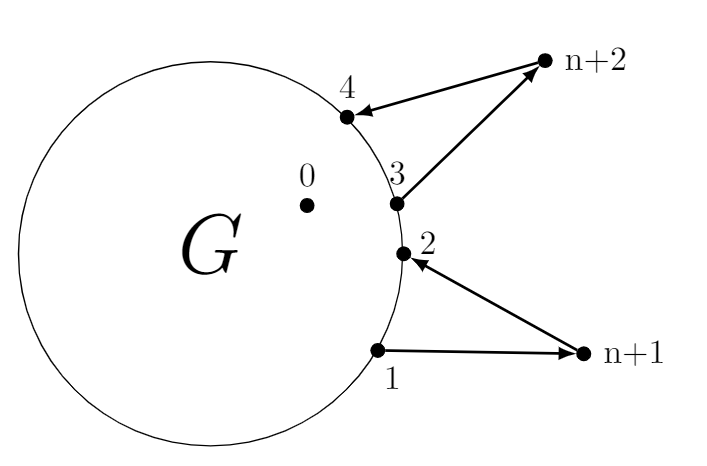
\includegraphics[scale=0.4]{tik_2handles.PNG}
\end{figure}
Then the number of spanning trees that are rooted at 1 in $VH_2(G)$ is
\begin{equation*}
    \begin{split}
        \tau_1(VH_2(G)) &= \tau(G)+\tau_{(1)(2)}(G)+\tau_{(3)(4)}(G)+
 \tau_{(13)(2)(4)}(G)+\tau_{(1)(23)(4)}(G)  \\
 & = \tau(G)+\tau_{(1)(2)}(G)+\tau_{(3)(4)}(G)+
 \tau_{(1)(2)(4)}(G)-\tau_{(1)(2)(43)}(G)
    \end{split}
\end{equation*}
\ethm

\bpf
Let $VH_2(G)$ be directed handle graph with 2 handles, and let $T$ be a spanning tree in $VH_2(G)$. Suppose $T$ is rooted at vertex $v_1\in V(G)$.Let $e_1$ be the inflow edge to node 2, and $e_2$ be the inflow edge to node 4. There are three cases.\\
Case 1. $e_1\notin VH_2(G)$ and $e_2\notin VH_2(G)$. Then by \Cref{bij_count} $$\tau_1(VH_2(G))=\tau(G)$$ 
Case 2. $e_1\in VH_2(G)$ and $e_2\notin VH_2(G)$. By \Cref{bij_count} and \Cref{addedW}, $$\tau_1(VH_2(G)) = \tau_{(1)(2)}(G)$$
Case 3. $e_1\notin VH_2(G)$ and $e_2\in VH(G)$.Similar to Case 2,  $$\tau_1(VH_2(G)) = \tau_{(3)(4)}(G)$$
Case 4. $e_1\in VH_2(G)$ and $e_2\in VH(G)$.\\
By \Cref{symhandle}, there is not exists a path between $v_1$ and $v_2$, nor a path between  $v_3$ and $v_4$. So, by \Cref{addedW}
$$\tau_1(VH_2(G)) = \tau_{(13)(2)(4)}(G)+\tau_{(1)(23)(4)}(G) = \tau_{(1)(2)(4)}(G)-\tau_{(1)(2)(43)}(G)$$
Therefore, the total number of spanning trees of $VH_2(G)$ is \begin{equation*}
    \begin{split}
        \tau_1(VH_2(G)) &= \tau(G)+\tau_{(1)(2)}(G)+\tau_{(3)(4)}(G)+
 \tau_{(13)(2)(4)}(G)+\tau_{(1)(23)(4)}(G)  \\
 & = \tau(G)+\tau_{(1)(2)}(G)+\tau_{(3)(4)}(G)+
 \tau_{(1)(2)(4)}(G)-\tau_{(1)(2)(43)}(G)
    \end{split}
\end{equation*}
\epf
% Leaving the graphical interpretations%
%Example of result%
%Wheel or butterfly graph%


\bthm\label{DH rooted 1 }
Let $H_2(G)$ be directed handle graph with 2 handles. Then the number of spanning trees that are rooted at 1 in $H_2(G)$ is
\begin{equation*}
    \begin{split}
        \tau_1(H_2(G)) &= \tau(G)+\tau_{(1)(2)}(G)+\tau_{(3)(4)}(G)+
 \tau_{(13)(2)(4)}(G)+\tau_{(1)(23)(4)}(G)  \\
 & = \tau(G)+\tau_{(1)(2)}(G)+\tau_{(3)(4)}(G)+
 \tau_{(1)(2)(4)}(G)-\tau_{(1)(2)(43)}(G)
    \end{split}
\end{equation*}
\ethm

\bpf
Let $H_2(G)$ be directed handle graph with 2 handles, and let $T$ be a spanning tree in $H_2(G)$. Suppose $T$ is rooted at vertex $v_1\in V(G)$.Let $e_1$ be the handle to node 2, and $e_2$ be the handle to node 4. There are three cases.\\
Case 1. $e_1\notin H_2(G)$ and $e_2\notin H_2(G)$. Then by \Cref{bij_count} $$\tau_1(H_2(G))=\tau(G)$$ 
Case 2. $e_1\in H_2(G)$ and $e_2\notin H_2(G)$. By \Cref{bij_count} and \Cref{addedW}, $$\tau_1(H_2(G)) = \tau_{(1)(2)}(G)$$
Case 3. $e_1\notin H_2(G)$ and $e_2\in H(G)$.Similar to Case 2,  $$\tau_1(H_2(G)) = \tau_{(3)(4)}(G)$$
Case 4. $e_1\in H_2(G)$ and $e_2\in H(G)$.\\
By \Cref{symhandle}, there is not exists a path between $v_1$ and $v_2$, nor a path between  $v_3$ and $v_4$. So, by \Cref{addedW}
$$\tau_1(VH_2(G)) = \tau_{(13)(2)(4)}(G)+\tau_{(1)(23)(4)}(G) = \tau_{(1)(2)(4)}(G)-\tau_{(1)(2)(43)}(G)$$
Therefore, the total number of spanning trees of $VH_2(G)$ is \begin{equation*}
    \begin{split}
        \tau_1(VH_2(G)) &= \tau(G)+\tau_{(1)(2)}(G)+\tau_{(3)(4)}(G)+
 \tau_{(13)(2)(4)}(G)+\tau_{(1)(23)(4)}(G)  \\
 & = \tau(G)+\tau_{(1)(2)}(G)+\tau_{(3)(4)}(G)+
 \tau_{(1)(2)(4)}(G)-\tau_{(1)(2)(43)}(G)
    \end{split}
\end{equation*}
\epf

%New Result
\bcor
Let $VH_2(G)$ be directed vertex handle graph with 2 handles. The number of 3-forests rooted at 1, 2, and 4 in $VH_2(G)$ is \[
\tau_{(1)(2)(43)}(G) = \tau(G)+\tau_{(1)(2)}(G)+\tau_{(3)(4)}(G)+
 \tau_{(1)(2)(4)}(G)-\tau_1(VH_2(G))
\]
Since we can calculate the exact number of spanning trees in each of $\tau(G)$,  $\tau_{(1)(2)}(G)$, $\tau_{(3)(4)}(G)$, $\tau_{(1)(2)(4)}(G)$, and $\tau_1(VH_2(G))$ using the Matrix Tree Theorem for digraph, we can calculate the exact number of 3-forests rooted at 1, 2, and 4 in $VH_2(G)$.
\ecor

The next corollary is a result!
\bcor
Let $H_2(G)$ be directed handle graph with 2 handles. The number of 3-forests rooted at 1, 2, and 4 in $H_2(G)$ is \[
\tau_{(1)(2)(43)}(G) = \tau(G)+\tau_{(1)(2)}(G)+\tau_{(3)(4)}(G)+
 \tau_{(1)(2)(4)}(G)-\tau_1(H_2(G))
\]
Since we can calculate the exact number of spanning trees in each of $\tau(G)$,  $\tau_{(1)(2)}(G)$, $\tau_{(3)(4)}(G)$, $\tau_{(1)(2)(4)}(G)$, and $\tau_1(H_2(G))$ using the Matrix Tree Theorem for digraph, we can calculate the exact number of 3-forests rooted at 1, 2, and 4 in $H_2(G)$.
\ecor


\subsubsection{Graphs with 2 handles rooted at 2}
\bthm
Let $VH_2(G)$ be directed vertex handle graph with 2 handles. 
\begin{figure}[H]
    \centering
    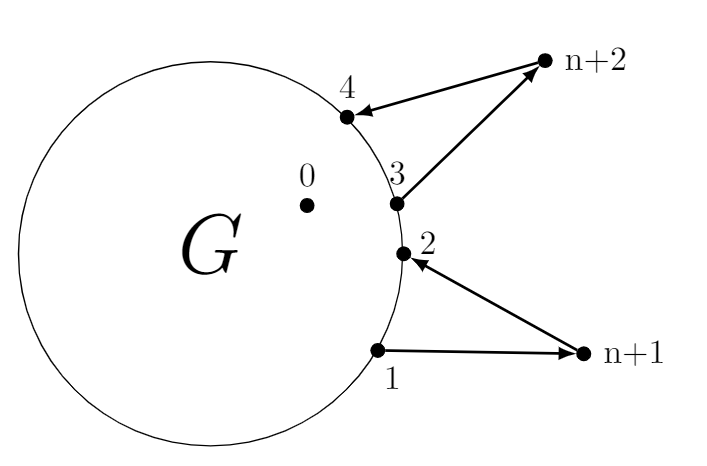
\includegraphics[scale=0.4]{tik_2handles.PNG}
\end{figure}
Then the number of spanning trees that are rooted at 2 in $VH_2(G)$ is  \[
\tau_2(VH_2(G)) = \tau(G) + \tau_{(3)(4)}(G)
\]
\ethm

\bpf
Let $VH_2(G)$ be directed handle graph with 2 handles, and let $t$ be a spanning tree in $VH_2(G)$. Suppose $t$ is rooted at 2. Let the inflow edge to $v_2$ be $e_1$ and the inflow edge to $v_4$ be $e_2$.\\
Case 1. $e_1 \notin VH_2(G)$ and $e_2 \notin VH_2(G)$.

Then by \Cref{bij_count} $\tau_2(VH_2(G))=\tau(G)$.\\
Case 2. $e_1 \in VH_2(G)$.

This contradicts with $T$ is rooted at $e_2$.\\
Case 3. $e_1\notin VH_2(G)$ and $e_2 \in VH_2(G)$.

By \Cref{symhandle}, there does not exist a path between $v_3$ and $v_4$. Then by \Cref{bij_count}, $\tau_2(VH_2(G)) = \tau_{(3)(4)}(G)$\\
Therefore, the total number of spanning trees in $VH_2(G)$ is \[
\tau_2(VH_2(G)) = \tau(G) + \tau_{(3)(4)}(G)
\]
\epf

\bthm\label{DH rooted 2 }
Let $H_2(G)$ be directed handle graph with 2 handles. Then the number of spanning trees that are rooted at 2 in $VH_2(G)$ is  \[
\tau_2(VH_2(G)) = \tau(G) + \tau_{(3)(4)}(G)
\]
\ethm

\bpf
Let $H_2(G)$ be directed handle graph with 2 handles, and let $t$ be a tree in $H_2(G)$. Suppose $t$ is rooted at 2. Let the inflow edge to $v_2$ be $e_1$ and the handle to $v_4$ be $e_2$.\\
Case 1. $e_1 \notin H_2(G)$ and $e_2 \notin H_2(G)$.

Then by \Cref{bij_count} $\tau_2(H_2(G))=\tau(G)$.\\
Case 2. $e_1 \in H_2(G)$.

This contradicts with $T$ is rooted at $e_2$.\\
Case 3. $e_1\notin H_2(G)$ and $e_2 \in H_2(G)$.

By \Cref{symhandle}, there does not exist a path between $v_3$ and $v_4$. Then by \Cref{bij_count}, $\tau_2(VH_2(G)) = \tau_{(3)(4)}(G)$\\
Therefore, the total number of spanning trees in $H_2(G)$ is \[
\tau_2(H_2(G)) = \tau(G) + \tau_{(3)(4)}(G)
\]
\epf

\subsubsection{Graphs with 2 handles rooted at 3}
\bthm
Let $VH_2(G)$ be directed vertex handle graph with 2 handles. 
\begin{figure}[H]
    \centering
    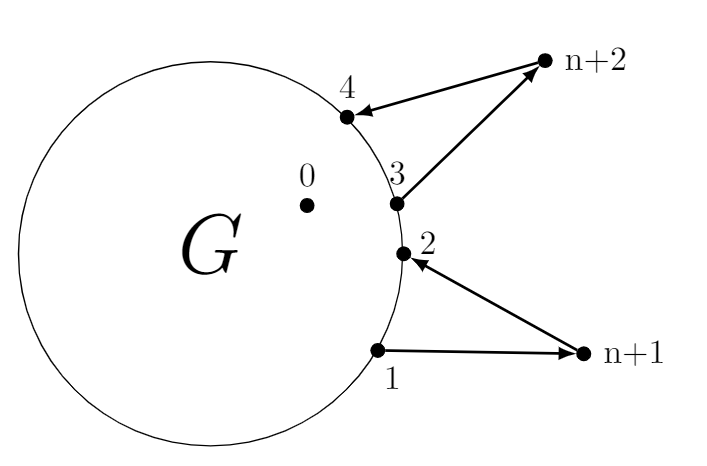
\includegraphics[scale=0.4]{tik_2handles.PNG}
\end{figure}
Then the number of spanning trees that are rooted at 3 in $VH_2(G)$ is
\begin{equation*}
    \begin{split}
        \tau_3(VH_2(G)) &= \tau(G)+\tau_{(1)(2)}(G)+\tau_{(3)(4)}(G)+
 \tau_{(31)(2)(4)}(G)+\tau_{(3)(2)(41)}(G)  \\
 &= \tau(G)+\tau_{(1)(2)}(G)+\tau_{(3)(4)}(G)+
 \tau_{(3)(2)(4)}(G)-\tau_{(3)(21)(4)}(G)
    \end{split}
\end{equation*}
\ethm
\bpf
Since graph rooted at 3 is symmetric to graph rooted at 1, by relabeling node 1, 3 and 2,4, we can get the result above.
\epf


\bthm\label{DH rooted 3} 
{\bf (Rooted at 3)}
Let $H_2(G)$ be directed handle graph with 2 handles. Then the number of spanning trees that are rooted at 3 in $H_2(G)$ is
\begin{equation*}
    \begin{split}
        \tau_3(VH_2(G)) &= \tau(G)+\tau_{(1)(2)}(G)+\tau_{(3)(4)}(G)+
 \tau_{(31)(2)(4)}(G)+\tau_{(3)(2)(41)}(G)  \\
 &= \tau(G)+\tau_{(1)(2)}(G)+\tau_{(3)(4)}(G)+
 \tau_{(3)(2)(4)}(G)-\tau_{(3)(21)(4)}(G)
    \end{split}
\end{equation*}
\ethm

\bpf
Since graph rooted at 3 is symmetric to graph rooted at 1, by relabeling node 1, 3 and 2,4, we can get the result above.
\epf

\subsubsection{Graphs with 2 handles rooted at 4}
\bthm
Let $VH_2(G)$ be directed vertex handle graph with 2 handles. 
\begin{figure}[H]
    \centering
    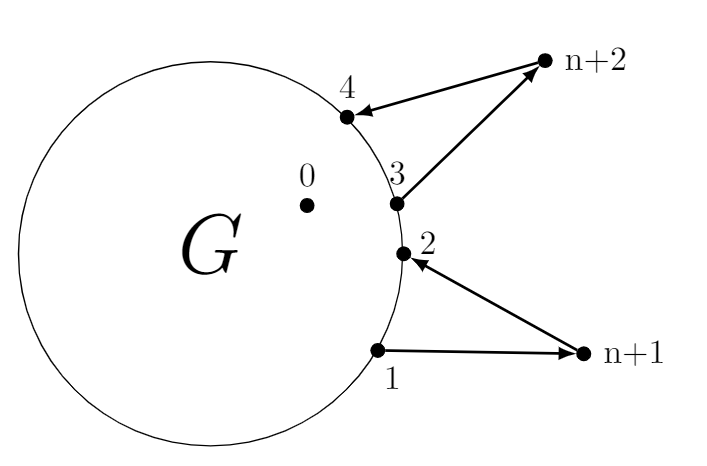
\includegraphics[scale=0.4]{tik_2handles.PNG}
\end{figure}
Then the number of spanning trees that are rooted at 4 in $VH_2(G)$ is \[
\tau_4(VH_2(G)) = \tau(G) + \tau_{(1)(2)}(G)
\]
\ethm
\bpf
Since graph rooted at 4 is symmetric to graph rooted at 2, by relabeling node 1, 3 and 2,4, we can get the result above.
\epf

\bthm\label{rooted 4} 

\ethm
{\bf (Rooted at 4)}
Let $H_2(G)$ be directed handle graph with 2 handles. Then the number of spanning trees that are rooted at 4 in $H_2(G)$ is \[
\tau_4(H_2(G)) = \tau(G) + \tau_{(1)(2)}(G)
\]
\bpf
Since graph rooted at 4 is symmetric to graph rooted at 2, by relabeling node 1, 3 and 2,4, we can get the result above.
\epf

\subsubsection{Graphs with 2 handles rooted at 0}
\bthm
Let $VH_2(G)$ be directed vertex handle graph with 2 handles.
\begin{figure}[H]
    \centering
    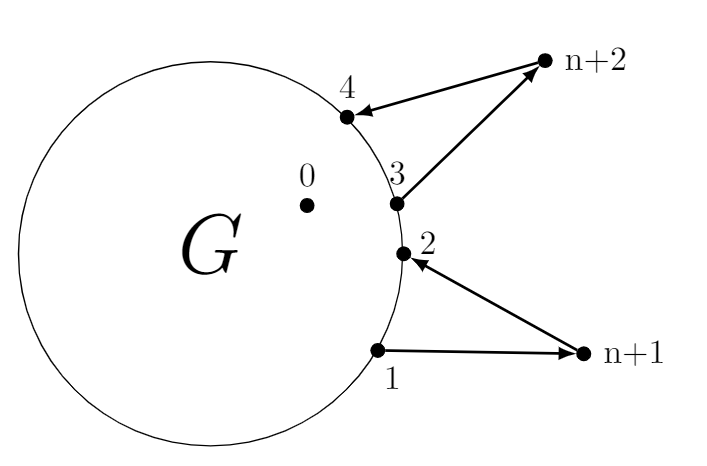
\includegraphics[scale=0.4]{tik_2handles.PNG}
\end{figure}
Then the number of spanning trees that are rooted at 0 in $VH_2(G)$ is
\begin{multline*}
\tau_0(VH_2(G)) = \tau(G) + \tau_{(1)(2)}(G)+ \tau_{(3)(4)}(G)\\ + \tau_{(013)(2)(4)}(G) + \tau_{(01)(23)(4)}(G) + \tau_{(03)(2)(14)}(G)
\end{multline*}
\ethm

\bpf
Let $VH_2(G)$ be directed vertex handle graph with 2 handles, and let $t$ be a spanning tree in $VH_2(G)$. Suppose $t$ is rooted at 0. Let the inflow edge to $v_2$ be $e_1$ and the inflow edge to $v_4$ be $e_2$.\\
Case 1. $e_1 \notin VH_2(G)$ and $e_2 \notin VH_2(G)$.Then by \Cref{bij_count},

$\tau_0(VH_2(G))=\tau(G)$\\
Case 2. Either $e_1 \in VH_2(G)$ or $e_2 \notin VH_2(G)$

By \Cref{symhandle}, there does not exist a path between $v_1$ and $v_2$ nor between $v_3$ and $v_4$. So,
$$\tau_0(VH_2(G))=\tau_{(1)(2)}(G)+ \tau_{(3)(4)}(G)$$ 
Case 4. $e_1\in VH_2(G)$ and $e_2 \in VH_2(G)$.

By \Cref{symhandle}, there does not exist a path between $v_1$ and $v_2$, and there does not exist a path between $v_3$ and $v_4$. So, $$\tau_0(VH_2(G))=\tau_{(013)(2)(4)}(G) + \tau_{(01)(23)(4)}(G) + \tau_{(03)(2)(14)}(G)$$
Combining three cases, the total number of spanning trees
\begin{multline*}
\tau_0(VH_2(G)) = \tau(G) + \tau_{(1)(2)}(G)+ \tau_{(3)(4)}(G)\\ + \tau_{(013)(2)(4)}(G) + \tau_{(01)(23)(4)}(G) + \tau_{(03)(2)(14)}(G)
\end{multline*}
\epf


\bthm \label{DH2 rooted at 0}
Let $H_2(G)$ be directed handle graph with 2 handles. Then the number of spanning trees that are rooted at 0 in $H_2(G)$ is
\begin{multline*}
\tau_0(H_2(G)) = \tau(G) + \tau_{(1)(2)}(G)+ \tau_{(3)(4)}(G)\\ + \tau_{(013)(2)(4)}(G) + \tau_{(01)(23)(4)}(G) + \tau_{(03)(2)(14)}(G)
\end{multline*}
\ethm

\bpf
Let $H_2(G)$ be directed handle graph with 2 handles, and let $t$ be a spanning tree in $H_2(G)$. Suppose $t$ is rooted at 0. Let the handle to $v_2$ be $e_1$ and the handle to $v_4$ be $e_2$.\\
Case 1. $e_1 \notin H_2(G)$ and $e_2 \notin H_2(G)$.Then by \Cref{bij_count},

$\tau_0(H_2(G))=\tau(G)$\\
Case 2. Either $e_1 \in H_2(G)$ or $e_2 \notin H_2(G)$

By \Cref{symhandle}, there does not exist a path between $v_1$ and $v_2$ nor between $v_3$ and $v_4$. So,
$$\tau_0(H_2(G))=\tau_{(1)(2)}(G)+ \tau_{(3)(4)}(G)$$ 
Case 4. $e_1\in H_2(G)$ and $e_2 \in H_2(G)$.

By \Cref{symhandle}, there does not exist a path between $v_1$ and $v_2$, and there does not exist a path between $v_3$ and $v_4$. So, $$\tau_0(H_2(G))=\tau_{(013)(2)(4)}(G) + \tau_{(01)(23)(4)}(G) + \tau_{(03)(2)(14)}(G)$$
Combining three cases, the total number of spanning trees
\begin{multline*}
\tau_0(H_2(G)) = \tau(G) + \tau_{(1)(2)}(G)+ \tau_{(3)(4)}(G)\\ + \tau_{(013)(2)(4)}(G) + \tau_{(01)(23)(4)}(G) + \tau_{(03)(2)(14)}(G)
\end{multline*}
\epf

\section{Results}

The following two results are our discoveries from this paper. For 1-handle graph, given any 2 vertices $v_1,v_2$ in the graph, we can relabel them as 1 and 2, respectively. By doing so, we can find the number of 2-forests rooted at these nodes. For 2-handle graph, given 4 vertices in the graph, we can find the number of 3-forests in the graph.

\begin{result}
Let $VH_1(G)$ be directed handle graph with 1 handle. Then the number of 2-forest rooted at 0 and 2 equals to the difference between the number of the spanning trees in $VH_1(G)$ and $G$. Moreover, using the Matrix Tree Theorem for digraphs, we can calculate the exact number for $\tau_{(01)(2)}(G)$.
\end{result}

\begin{result}
Let $VH_2(G)$ be a directed handle graph with 2 handles. The number of 3-forests rooted at 1, 2, and 4 in $VH_2(G)$ is \[
\tau_{(1)(2)(43)}(G) = \tau(G)+\tau_{(1)(2)}(G)+\tau_{(3)(4)}(G)+
 \tau_{(1)(2)(4)}(G)-\tau_1(VH_2(G))
\]
Since we can calculate the exact number of spanning trees in each of $\tau(G)$,  $\tau_{(1)(2)}(G)$, $\tau_{(3)(4)}(G)$, $\tau_{(1)(2)(4)}(G)$, and $\tau_1(VH_2(G))$ using the Matrix Tree Theorem for digraph, we can calculate the exact number of 3-forests rooted at 1, 2, and 4 in $VH_2(G)$.
\end{result}

%\section{References}

\subsection{Future exploration of Graphs with 3 handles}

Such as with the growth from one handles to two handles started to increase the number of directed spanning trees, so it will be with the increase from 2 handles to 3 handles, in addition the amount of growth of trees increases.

\subsubsection{Graphs with 3 handles rooted at 1}
\bthm
Let $VH_3(G)$ be directed vertex handle graph with 3 handles.
\begin{figure}[H]
    \centering
    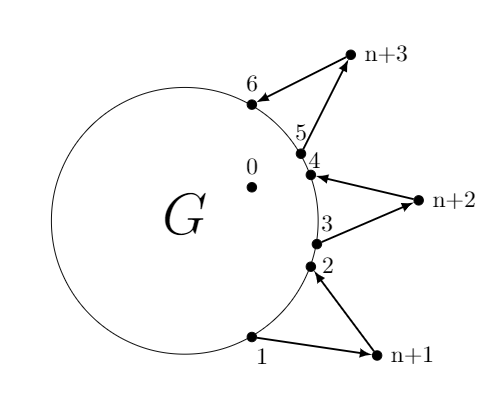
\includegraphics[scale=0.4]{tik_3handles.PNG}
\end{figure}
Then the number of spanning trees that are rooted at 1 in $VH_3(G)$ is
\begin{equation*}
    \begin{split}
        \tau_1(VH_3(G)) &= \tau(G) + \tau_{(1)(2)}(G)+ \tau_{(3)(4)}(G) + \tau_{(5)(6)}(G)\\ 
        &+ \tau_{(13)(2)(4)}(G) + \tau_{(1)(23)(4)}(G) + \tau_{(15)(2)(6)}(G) + \tau_{(1)(25)(6)}(G)\\
        &+ \tau_{(135)(4)(6)}(G) + \tau_{(13)(45)(6)}(G) + \tau_{(15)(36)(4)}(G)\\
        &+ \tau_{(135)(2)(4)(6)}(G) + \tau_{(13)(2)(45)(6)}(G) + \tau_{(13)(25)(4)(6)}(G)\\
&+ \tau_{(15)(2)(4)(36)}(G) + \tau_{(15)(23)(4)(6)}(G)
    \end{split}
\end{equation*}
\ethm

\bthm \label{DH rooted at 1}
Let $H_3(G)$ be directed handle graph with 3 handles. Then the number of spanning trees that are rooted at 1 in $H_3(G)$ is
\begin{equation*}
    \begin{split}
        \tau_1(H_3(G)) &= \tau(G) + \tau_{(1)(2)}(G)+ \tau_{(3)(4)}(G) + \tau_{(5)(6)}(G)\\ 
        &+ \tau_{(13)(2)(4)}(G) + \tau_{(1)(23)(4)}(G) + \tau_{(15)(2)(6)}(G) + \tau_{(1)(25)(6)}(G)\\
        &+ \tau_{(135)(4)(6)}(G) + \tau_{(13)(45)(6)}(G) + \tau_{(15)(36)(4)}(G)\\
        &+ \tau_{(135)(2)(4)(6)}(G) + \tau_{(13)(2)(45)(6)}(G) + \tau_{(13)(25)(4)(6)}(G)\\
&+ \tau_{(15)(2)(4)(36)}(G) + \tau_{(15)(23)(4)(6)}(G)
    \end{split}
\end{equation*}
\ethm

\subsubsection{Graphs with 3 handles rooted at 2}
\bthm
Let $VH_3(G)$ be directed vertex handle graph with 3 handles.
\begin{figure}[H]
    \centering
    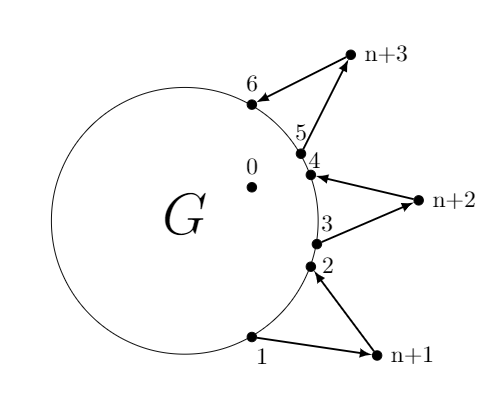
\includegraphics[scale=0.4]{tik_3handles.PNG}
\end{figure}
Then the number of spanning trees that are rooted at 2 in $VH_3(G)$ is
\[
\tau_2(VH_3(G)) = \tau(G) + \tau_{(3)(4)}(G) + \tau_{(5)(6)}(G) + \tau_{(3)(45)(6)}(G)+ \tau_{(35)(4)(6)}(G)
\]
\ethm

\bthm
Let $H_3(G)$ be directed handle graph with 3 handles. Then the number of spanning trees that are rooted at 2 in $H_3(G)$ is
\[
\tau_2(H_3(G)) = \tau(G) + \tau_{(3)(4)}(G) + \tau_{(5)(6)}(G) + \tau_{(3)(45)(6)}(G)+ \tau_{(35)(4)(6)}(G)
\]
\ethm

\subsubsection{Graphs with 3 handles rooted at 3}
\bthm
Let $VH_3(G)$ be directed vertex handle graph with 3 handles. 
\begin{figure}[H]
    \centering
    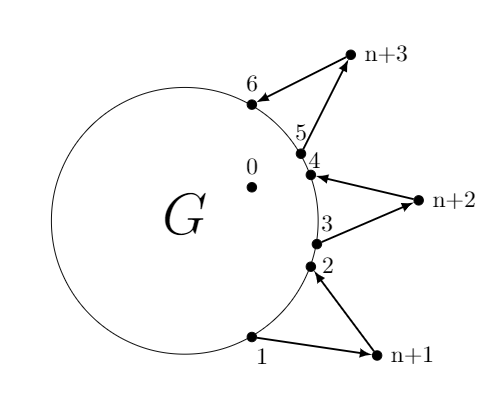
\includegraphics[scale=0.4]{tik_3handles.PNG}
\end{figure}
Then the number of spanning trees that are rooted at 3 in $VH_3(G)$ is
\begin{equation*}
    \begin{split}
        \tau_3(VH_3(G)) &= \tau(G) + \tau_{(1)(2)}(G)+ \tau_{(3)(4)}(G) + \tau_{(5)(6)}(G)\\ 
        &+ \tau_{(35)(4)(6)}(G) + \tau_{(3)(45)(6)}(G) + \tau_{(13)(2)(4)}(G) + \tau_{(3)(14)(2)}(G)\\
        &+ \tau_{(135)(2)(6)}(G) + \tau_{(35)(16)(2)}(G) + \tau_{(13)(25)(6)}(G)\\
        &+ \tau_{(135)(2)(4)(6)}(G) + \tau_{(35)(16)(2)(4)}(G) + \tau_{(35)(14)(2)(6)}(G)\\
&+ \tau_{(13)(25)(6)(4)}(G) + \tau_{(13)(45)(2)(6)}(G)
    \end{split}
\end{equation*}
\ethm

\bthm
Let $H_3(G)$ be directed handle graph with 3 handles. Then the number of spanning trees that are rooted at 3 in $H_3(G)$ is
\begin{equation*}
    \begin{split}
        \tau_3(H_3(G)) &= \tau(G) + \tau_{(1)(2)}(G)+ \tau_{(3)(4)}(G) + \tau_{(5)(6)}(G)\\ 
        &+ \tau_{(35)(4)(6)}(G) + \tau_{(3)(45)(6)}(G) + \tau_{(13)(2)(4)}(G) + \tau_{(3)(14)(2)}(G)\\
        &+ \tau_{(135)(2)(6)}(G) + \tau_{(35)(16)(2)}(G) + \tau_{(13)(25)(6)}(G)\\
        &+ \tau_{(135)(2)(4)(6)}(G) + \tau_{(35)(16)(2)(4)}(G) + \tau_{(35)(14)(2)(6)}(G)\\
&+ \tau_{(13)(25)(6)(4)}(G) + \tau_{(13)(45)(2)(6)}(G)
    \end{split}
\end{equation*}
\ethm

\subsubsection{Graphs with 3 handles rooted at 4}
\bthm
Let $VH_3(G)$ be directed handle graph with 3 handles.
\begin{figure}[H]
    \centering
    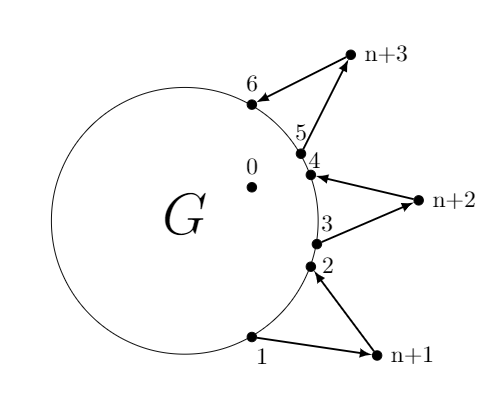
\includegraphics[scale=0.4]{tik_3handles.PNG}
\end{figure}
Then the number of spanning trees that are rooted at 4 in $VH_3(G)$ is
\[
\tau_4(VH_3(G)) = \tau(G) + \tau_{(1)(2)}(G)+ \tau_{(5)(6)}(G) + \tau_{(1)(25)(6)}(G)+ \tau_{(15)(2)(6)}(G)
\]
\ethm

\bthm
Let $H_3(G)$ be directed handle graph with 3 handles. Then the number of spanning trees that are rooted at 4 in $H_3(G)$ is
\[
\tau_4(H_3(G)) = \tau(G) + \tau_{(1)(2)}(G)+ \tau_{(5)(6)}(G) + \tau_{(1)(25)(6)}(G)+ \tau_{(15)(2)(6)}(G)
\]
\ethm

\subsubsection{Graphs with 3 handles rooted at 5}
\bthm
Let $VH_3(G)$ be directed vertex handle graph with 3 handles.
\begin{figure}[H]
    \centering
    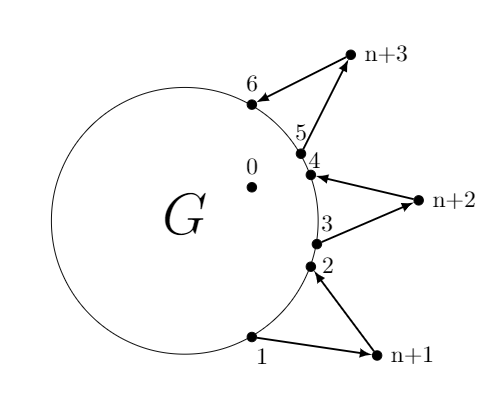
\includegraphics[scale=0.4]{tik_3handles.PNG}
\end{figure}
Then the number of spanning trees that are rooted at 5 in $VH_3(G)$ is
\begin{equation*}
    \begin{split}
        \tau_5(VH_3(G)) &= \tau(G) + \tau_{(1)(2)}(G)+ \tau_{(3)(4)}(G) + \tau_{(5)(6)}(G)\\ 
        &+ \tau_{(53)(4)(6)}(G) + \tau_{(5)(36)(4)}(G) + \tau_{(15)(2)(6)}(G) + \tau_{(5)(16)(2)}(G)\\
        &+ \tau_{(135)(2)(4)}(G) + \tau_{(15)(23)(4)}(G) + \tau_{(35)(14)(2)}(G)\\
        &+ \tau_{(135)(2)(4)(6)}(G) + \tau_{(15)(23)(4)(6)}(G) + \tau_{(15)(36)(2)(4)}(G)\\
&+ \tau_{(35)(14)(2)(6)}(G) + \tau_{(35)(16)(2)(4)}(G)
    \end{split}
\end{equation*}
\ethm

\bthm
Let $H_3(G)$ be directed handle graph with 3 handles. Then the number of spanning trees that are rooted at 5 in $H_3(G)$ is
\begin{equation*}
    \begin{split}
        \tau_5(H_3(G)) &= \tau(G) + \tau_{(1)(2)}(G)+ \tau_{(3)(4)}(G) + \tau_{(5)(6)}(G)\\ 
        &+ \tau_{(53)(4)(6)}(G) + \tau_{(5)(36)(4)}(G) + \tau_{(15)(2)(6)}(G) + \tau_{(5)(16)(2)}(G)\\
        &+ \tau_{(135)(2)(4)}(G) + \tau_{(15)(23)(4)}(G) + \tau_{(35)(14)(2)}(G)\\
        &+ \tau_{(135)(2)(4)(6)}(G) + \tau_{(15)(23)(4)(6)}(G) + \tau_{(15)(36)(2)(4)}(G)\\
&+ \tau_{(35)(14)(2)(6)}(G) + \tau_{(35)(16)(2)(4)}(G)
    \end{split}
\end{equation*}
\ethm

\subsubsection{Graphs with 3 handles rooted at 6}
\bthm
Let $VH_6(G)$ be directed vertex handle graph with 3 handles. 
\begin{figure}[H]
    \centering
    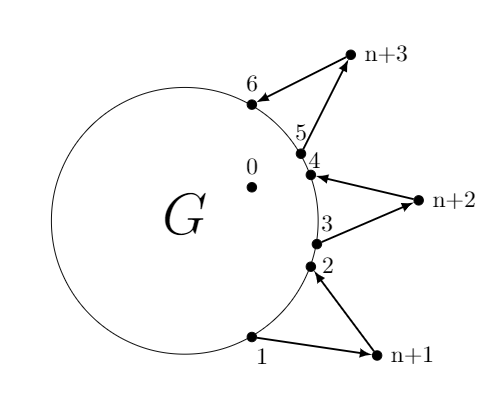
\includegraphics[scale=0.4]{tik_3handles.PNG}
\end{figure}
Then the number of spanning trees that are rooted at 6 in $VH_3(G)$ is
\[
\tau_6(VH_3(G)) = \tau(G) + \tau_{(1)(2)}(G)+ \tau_{(3)(4)}(G) + \tau_{(1)(23)(4)}(G)+ \tau_{(13)(2)(4)}(G)
\]
\ethm

\bthm
Let $H_6(G)$ be directed handle graph with 3 handles. Then the number of spanning trees that are rooted at 6 in $H_3(G)$ is
\[
\tau_6(H_3(G)) = \tau(G) + \tau_{(1)(2)}(G)+ \tau_{(3)(4)}(G) + \tau_{(1)(23)(4)}(G)+ \tau_{(13)(2)(4)}(G)
\]
\ethm

\subsubsection{Graphs with 3 handles rooted at 0}
\bthm
Let $H_3(G)$ be directed vertex handle graph with 3 handles. 
\begin{figure}[H]
    \centering
    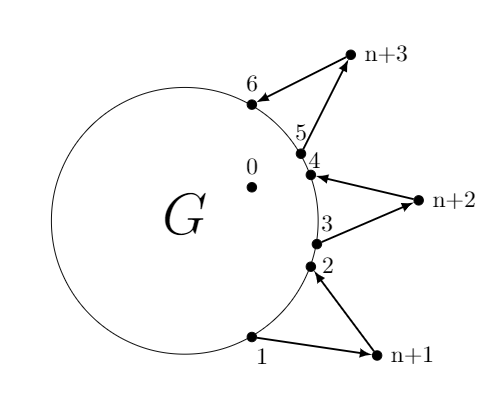
\includegraphics[scale=0.4]{tik_3handles.PNG}
\end{figure}
Then the number of spanning trees that are rooted at 0 in $VH_3(G)$ is
\begin{equation*}
    \begin{split}
        \tau_0(H_3(G)) &= \tau(G) + \tau_{(1)(2)}(G)+ \tau_{(3)(4)}(G) + \tau_{(5)(6)}(G)\\ 
        &+ \tau_{(01)(23)(4)}(G) + \tau_{(03)(14)(2)}(G) + \tau_{(013)(2)(4)}(G)\\
        &+ \tau_{(03)(24)(6)}(G) + \tau_{(05)(4)(36)}(G) + \tau_{(035)(4)(6)}(G)\\
        &+ \tau_{(01)(25)(6)}(G) + \tau_{(05)(2)(16)}(G) + \tau_{(015)(2)(6)}(G)\\
        &+ \tau_{(0135)(2)(4)(6)}(G) + \tau_{(013)(25)(4)(6)}(G) + \tau_{(013)(45)(2)(6)}(G)\\
        &+ \tau_{(015)(23)(4)(6)}(G) + \tau_{(015)(36)(2)(4)}(G) + \tau_{(035)(41)(2)(6)}(G) + \tau_{(035)(61)(2)(4)}(G)\\
        &+ \tau_{(01)(23)(45)(6)}(G) + \tau_{(01)(25)(36)(4)}(G) + \tau_{(01)(235)(4)(6)}(G)\\
        &+ \tau_{(03)(45)(16)(2)}(G) + \tau_{(03)(14)(25)(6)}(G) + \tau_{(03)(145)(2)(6)}(G)\\
        &+ \tau_{(05)(16)(23)(4)}(G) + \tau_{(05)(36)(14)(2)}(G) + \tau_{(05)(163)(2)(4)}(G)
    \end{split}
\end{equation*}
\ethm

\bthm
Let $H_3(G)$ be directed handle graph with 3 handles. Then the number of spanning trees that are rooted at 0 in $H_3(G)$ is
\begin{equation*}
    \begin{split}
        \tau_0(H_3(G)) &= \tau(G) + \tau_{(1)(2)}(G)+ \tau_{(3)(4)}(G) + \tau_{(5)(6)}(G)\\ 
        &+ \tau_{(01)(23)(4)}(G) + \tau_{(03)(14)(2)}(G) + \tau_{(013)(2)(4)}(G)\\
        &+ \tau_{(03)(24)(6)}(G) + \tau_{(05)(4)(36)}(G) + \tau_{(035)(4)(6)}(G)\\
        &+ \tau_{(01)(25)(6)}(G) + \tau_{(05)(2)(16)}(G) + \tau_{(015)(2)(6)}(G)\\
        &+ \tau_{(0135)(2)(4)(6)}(G) + \tau_{(013)(25)(4)(6)}(G) + \tau_{(013)(45)(2)(6)}(G)\\
        &+ \tau_{(015)(23)(4)(6)}(G) + \tau_{(015)(36)(2)(4)}(G) + \tau_{(035)(41)(2)(6)}(G) + \tau_{(035)(61)(2)(4)}(G)\\
        &+ \tau_{(01)(23)(45)(6)}(G) + \tau_{(01)(25)(36)(4)}(G) + \tau_{(01)(235)(4)(6)}(G)\\
        &+ \tau_{(03)(45)(16)(2)}(G) + \tau_{(03)(14)(25)(6)}(G) + \tau_{(03)(145)(2)(6)}(G)\\
        &+ \tau_{(05)(16)(23)(4)}(G) + \tau_{(05)(36)(14)(2)}(G) + \tau_{(05)(163)(2)(4)}(G)
    \end{split}
\end{equation*}
\ethm

\section{Future Work}

We conjecture that there are similar relationships in the exploration of counting the number of spanning trees and $n-$forests in the 3-handle graph. This will allow us to count the number of 3-forests in the 3-handle graph.


\begin{thebibliography}{20}

\bibitem{Lap} Goldberg, L.; Matrix Theory with Applications. McGraw-Hill International Editions, \emph{Mathematics and Statistics Series} (1991).

\bibitem{GP} Gyurov, B.; Pinzon,D.; The Determinant of Graphs Joined by j-edges. \emph{The Thai Journal of Mathematics}. Aug. 2015.

\bibitem{H} Harary, F.; The Determinant of the adjacency matrix of a graph. \emph{SIAM Rev.}, \textbf{4} (1961), 202 - 210.

\bibitem{leenheer} Leenheer, P.; An elementary proof of a matrix tree theorem for directed graphs. \emph{arXiv e-prints}, April, 2012.

\bibitem{Mar} Margoliash, J.;
Matrix-Tree Theorem for Directed Graphs.  \emph{SIAM Journal of Discrete Mathematics}, \textbf{3}(1) (1990), 7 - 20.

\bibitem{BG} Sookyang,S.; Arworn, S.; Gyurov, B.;  Determinant of Graphs joined by two edges. \emph{The Thai Journal of Mathematics}, \textbf{10} (2012) 1: 101-111.

\end{thebibliography}
\end{document}